% --------------------------------------------------------------
% This is all preamble stuff that you don't have to worry about.
% Head down to where it says "Start here"
% --------------------------------------------------------------

\documentclass[12pt]{article}

\usepackage[margin=1in]{geometry}
\usepackage{amsmath,amsthm,amssymb}
\usepackage{tikz}

\newcommand{\N}{\mathbb{N}}
\newcommand{\Z}{\mathbb{Z}}

\newenvironment{theorem}[2][Theorem]{\begin{trivlist}
\item[\hskip \labelsep {\bfseries #1}\hskip \labelsep {\bfseries #2.}]}{\end{trivlist}}
\newenvironment{lemma}[2][Lemma]{\begin{trivlist}
\item[\hskip \labelsep {\bfseries #1}\hskip \labelsep {\bfseries #2.}]}{\end{trivlist}}
\newenvironment{exercise}[2][Exercise]{\begin{trivlist}
\item[\hskip \labelsep {\bfseries #1}\hskip \labelsep {\bfseries #2.}]}{\end{trivlist}}
\newenvironment{question}[2][Question]{\begin{trivlist}
\item[\hskip \labelsep {\bfseries #1}\hskip \labelsep {\bfseries #2.}]}{\end{trivlist}}
\newenvironment{proposition}[2][Proposition]{\begin{trivlist}
\item[\hskip \labelsep {\bfseries #1}\hskip \labelsep {\bfseries #2.}]}{\end{trivlist}}
\newenvironment{corollary}[2][Corollary]{\begin{trivlist}
\item[\hskip \labelsep {\bfseries #1}\hskip \labelsep {\bfseries #2.}]}{\end{trivlist}}

\begin{document}

% --------------------------------------------------------------
%                         Start here
% --------------------------------------------------------------

%\renewcommand{\qedsymbol}{\filledbox}

\title{Homework 3}%replace X with the appropriate number
\author{Dustin Lambright - dalambri \\ Aseem Raina - araina \\ Bihan Zhang - bzhang28 \\ Anshul Fadnavis - asfadnav\\
%replace with your name
CSC 565 - Graph Theory} %if necessary, replace with your course title

\maketitle


\begin{question}{1}
Show that every simple graph $G$ with 6 vertices has either a clique of size 3 or an independent
set of size 3.
\end{question}

By the definition of independent sets and cliques, any graph G with a clique of size n will also have a clique of n-1, n-2, ... n-(n-1).  The same goes for an independent set.  Therefore, using contradiction, if a graph does not have a clique of size 3 and does not have an independent set of size 3, the statement is false. \\ \\

The graph $K_{1,5}$ has a maximum clique size of 2, but an independent set of 5. (displayed in red)
\begin{align*}
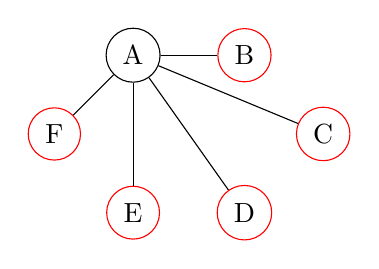
\begin{tikzpicture}
\node[shape=circle,draw=black] (A) at (1,2) {A};
\node[shape=circle,draw=red] (B) at (2.4142857,2) {B};
\node[shape=circle,draw=red] (C) at (3.4142856,1) {C};
\node[shape=circle,draw=red] (D) at (2.4142857,0) {D};
\node[shape=circle,draw=red] (E) at (1,0) {E};
\node[shape=circle,draw=red] (F) at (0,1) {F};
\path [] (A) edge node[left] {} (B);
\path [] (A) edge node[left] {} (C);
\path [] (A) edge node[left] {} (D);
\path [] (A) edge node[left] {} (E);
\path [] (A) edge node[left] {} (F);
\end{tikzpicture}
\end{align*}

In an effort to reduce the size of the maximum independent set, edges are replaced, creating a cyclic graph: \\

\begin{align*}
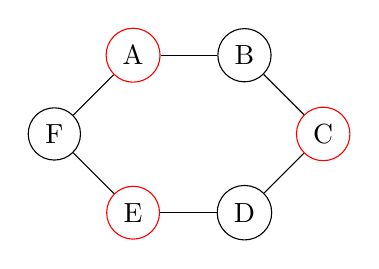
\begin{tikzpicture}
\node[shape=circle,draw=red] (A) at (1,2) {A};
\node[shape=circle,draw=black] (B) at (2.4142857,2) {B};
\node[shape=circle,draw=red] (C) at (3.4142856,1) {C};
\node[shape=circle,draw=black] (D) at (2.4142857,0) {D};
\node[shape=circle,draw=red] (E) at (1,0) {E};
\node[shape=circle,draw=black] (F) at (0,1) {F};
\path [] (A) edge node[left] {} (B);
\path [] (B) edge node[left] {} (C);
\path [] (C) edge node[left] {} (D);
\path [] (D) edge node[left] {} (E);
\path [] (F) edge node[left] {} (A);
\path [] (E) edge node[left] {} (F);
\end{tikzpicture}
\end{align*}

This graph has a a maximum independent set of 3, and a maximum clique of 2. The only way to reduce the size of an independent set, i.e., $\{A,E,C\}$ is to connect any of those vertices with an edge.  The connection of any of these vertices results in a clique of size 3.  In an effort to maintain our clique constraint, if we remove the edges AF and AB to connect the independent set $\{A,E,C\}$, we end up with an independent set $\{A,F,B, D\}$.

\begin{align*}
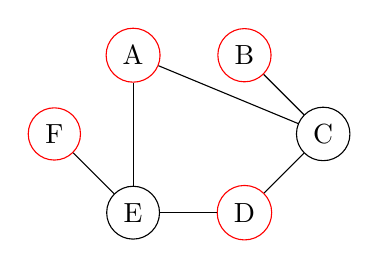
\begin{tikzpicture}
\node[shape=circle,draw=red] (A) at (1,2) {A};
\node[shape=circle,draw=red] (B) at (2.4142857,2) {B};
\node[shape=circle,draw=black] (C) at (3.4142856,1) {C};
\node[shape=circle,draw=red] (D) at (2.4142857,0) {D};
\node[shape=circle,draw=black] (E) at (1,0) {E};
\node[shape=circle,draw=red] (F) at (0,1) {F};
\path [] (A) edge node[left] {} (C);
\path [] (B) edge node[left] {} (C);
\path [] (C) edge node[left] {} (D);
\path [] (D) edge node[left] {} (E);
\path [] (E) edge node[left] {} (A);
\path [] (E) edge node[left] {} (F);
\end{tikzpicture}
\end{align*}

The graph $C_6$ is the closest we can get to a graph without a clique of size 3 and without an independent set of size 3, but it has an independent set of size three, proving that a graph with a vertex count of 6 has to have an independent set of size 3 or a clique of size 3.

\begin{question}{2}
Prove or disprove: In a simple graph, every closed even trail of length more than 3 contains an even cycle.
\begin{align*}
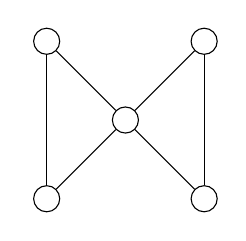
\begin{tikzpicture}
\node[shape=circle,draw=black] (B) at (1,0) {};
\node[shape=circle,draw=black] (D) at (1,-2) {};
\node[shape=circle,draw=black] (E) at (2,-1) {};
\node[shape=circle,draw=black] (F) at (3,0) {};
\node[shape=circle,draw=black] (H) at (3,-2) {};
\path [] (B) edge node[left] {} (E);
\path [] (D) edge node[left] {} (E);
\path [] (E) edge node[left] {} (F);
\path [] (H) edge node[left] {} (E);
\path [] (B) edge node[left] {} (D);
\path [] (F) edge node[left] {} (H);
\end{tikzpicture}
\end{align*}
\end{question}

\begin{question}{3}
Prove the following by strong induction on the length of the trail: The edge set of every closed trail can be partitioned into one or more pairwise edge-disjoint cycles.
\end{question}

\textbf{i.} The edge set $E$ of every closed trail can be partitioned into one or more pairwise edge-disjoint cycles\\

Proof: Let $G$ be the graph containing the edge set $E$. \\

Let $n$ be the length of the maximum closed trial in $G$ of the form ($v_1$, $v_2$), ... ($v_n$, $v_1$). \\

Let $C$ be the smallest cycle in $G$ of the form ($v_i$, $v_{i+1}$)...($v_{i+k-1}$, $v_{i+k}$), where $v_i = v_{i+k}$ and $v_i$...$v_{i+k-1}$ are distinct (if the vertexes were not distinct that would mean it would be able to be partitioned into smaller cycles, and we started this exercise assuming C is the smallest cycle). \\

If $C = G$, the graph can be partitioned into one pairwise edge-disjoint cycle.\\

Otherwise, Let $G' = G - C$\\

The length of the closed trial through $G'$ cannot be more than $n$, and would have the closed trial ($v_1$, $v_2$)...($v_n$, $v_1$). \\

By induction we can partition the edge set of $G'$ into smaller disjoint cycles. Thus we show that the edge set of $G$ can be partitioned into disjoint cycles consisting of all the cycles in $G'$ and $C$\\

\textbf{ii.} If an edge set $E$ can be partitioned into one or more pairwise edge-disjoint cycles, it is a closed trial. \\

Proof: Let $G$ be the graph containing the edge set $E$.\\

If the edge set of $G$ can be partitioned into pairwise edge-disjoint cycles, every vertex must have an even degree (for v to be on a cycle it must have 2 degrees). Since every vertex is even $G$ must be Eulerian by Theorem 1.2.26. Every Eulerian graph must have a closed trial. Thus $G$ must have a closed trial.

\begin{question}{4}
Suppose that $T$ is a maximal trail in a simple graph $G$ and that $T$ has at least one edge and is not closed. Prove that the endpoints of T have odd degree.
\end{question}

Let $v_1$ and $v_n$ be the endpoints of $T$ (it must have at least 2 distinct vertexes, since it has at least one edge, and is not closed.). \\

Since $T$ is not closed, $v_1$ and $v_n$ cannot be connected. \\

If $v_1$ had a neighbors $v_0$, and their connected edge was not in $T$, it must be added in $T$ in order for $T$ to be maximal. Thus $v_1$ can only have one neighbor $v_2$. And any vertex, on a simple graph, with one neighbor has a degree of 1. The same argument can be applied to $v_n$ showing that it, also, has a degree of 1.

\begin{question}{5}
If G is a graph with vertices v1, v2, . . . , vn and Ak denotes the kth power of the adjacency matrix
of G under matrix multiplication then \\ \\
(***) $A^{k}[i, j]$ is the number of vi, vj -walks of length k in G. \\ \\
Show how to use (***) to solve the following without multipltying matrices and prove your answer
correct: Let A be the adjacency matrix of Kn. If i = j, then A3
[i, j] =\_\_\_\_ . Otherwise
A3
[i, j] = \_\_\_\_.
\end{question}

\begin{question}{6}
Draw a simple, connected graph with the following degree sequence, or prove that no such graph
is possible: \\
a. (3, 3, 3, 2, 2, 2) \\
For any graph G, the number of vertices of odd degree should be even. Here, we have 3 vertices of odd degree (3,3,3), hence no such graph is possible. \\
b. (7, 6, 5, 4, 3, 2, 1) \\
No such graph is possible as a vertex cannot have degree equal to the total number of
vertices in the graph (i.e. 7). \\ \\
c. (3, 3, 2, 2, 1, 1) \\
A graph is possible \\
\begin{align*}
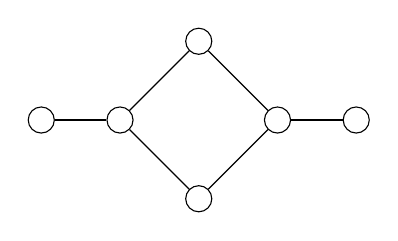
\begin{tikzpicture}
\node[shape=circle,draw=black] (A) at (-1,0) {};
\node[shape=circle,draw=black] (B) at (0,1) {};
\node[shape=circle,draw=black] (C) at (1,0) {};
\node[shape=circle,draw=black] (D) at (0,-1) {};
\node[shape=circle,draw=black] (E) at (-2,0) {};
\node[shape=circle,draw=black] (F) at (2,0) {};
\path [] (A) edge node[left] {} (B);
\path [] (B) edge node[left] {} (C);
\path [] (C) edge node[left] {} (D);
\path [] (D) edge node[left] {} (A);
\path [] (A) edge node[left] {} (E);
\path [] (C) edge node[left] {} (F);
\end{tikzpicture}
\end{align*}
d. (7, 6, 5, 4, 3, 3, 2) \\
No such graph is possible as a vertex cannot have degree equal to the total number of
vertices in the graph (i.e. 7). \\
e. (6, 6, 5, 4, 3, 3, 1)
No such graph is possible as two vertices cannot have degree 6 for the following sequence.
\end{question}

\begin{question}{7}
 How many different simple graphs are there with 5 edges and with vertex set {v1, v2, . . . v5}?
(We are counting labeled graphs, not isomorphism classes)
For an edge, we need to choose 2 vertices out of 5, which can be done in ${5 \choose 2}$ ways. The total number of such edge subsets is $2^{5 \choose 2} = 2^{10} = 1024$ graphs.
\end{question}

\begin{question}{8}
Prove by contradiction: A graph with every vertex degree even has no cut-edge.
\end{question}




% --------------------------------------------------------------
%     You don't have to mess with anything below this line.
% --------------------------------------------------------------

\end{document}
